\documentclass{standalone}
\usepackage{tikz,pgfplots,calc}
\usetikzlibrary{positioning,calc}
\usetikzlibrary{arrows}
\usepackage{tkz-euclide}
\usetkzobj{all}


\begin{document}
\begin{tikzpicture}[>=stealth', thick]
    \node [label = below: Iris setosa] (n1) at (0, 0) {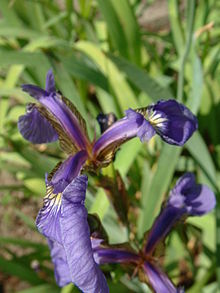
\includegraphics[height = 100pt]{iris1.jpg}};
    \node (n2) [anchor = west, right = -5pt of n1.east, label = below: Iris versicolor] {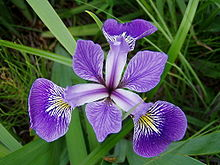
\includegraphics[height = 100pt]{iris2.jpg}};
    \node (n3) [anchor = west, right = -5pt of n2.east, label = below: Iris virginica] {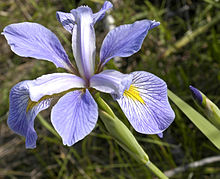
\includegraphics[height = 100pt]{iris3.jpg}};
\end{tikzpicture}
\end{document}